% Designed for LuaLaTex

\documentclass[12pt]{article}
\usepackage{graphicx,amssymb, amstext, amsmath, epstopdf, booktabs, verbatim, gensymb, geometry, appendix, natbib, lmodern, url, titlesec, tabularx, array, enumitem}
\usepackage[hyperfootnotes=false]{hyperref}
\setlist[enumerate]{itemsep=0mm}
\setlist[itemize]{itemsep=0mm}
\geometry{letterpaper}
%\usepackage{garamond}

\newcommand*\Title{Ttitle goes here}
\newcommand*\cpiType{Subtitle goes here}
\newcommand*\Date{Date goes here}
\newcommand{\version}{0.1}
\title{Title goes here}
\newcolumntype{R}{>{\raggedright\arraybackslash\small}X}%
\date{Date goes here}
%-----------------------------------------------------------

\usepackage{oe-assets/oe} % This is what makes your document look like a cpi document.


\begin{document}
% \begin{titlepage}
\maketitle
% \end{titlepage}
\pagebreak
\hfill
\vspace{86pt}
\begin{center}
[ This page intentionally left blank]
\end{center}
\pagebreak


\begin{spacing}{1}
\pagenumbering{roman}
\noindent
CC BY-SA 2.5 CA 2016 Open Effect.
\hfill \break
\hfill \break
Electronic version first published at openeffect.ca in 2016 by Open Effect. Open Effect is a Canadian not-for-profit applied research organization focusing on digital privacy and security. 
\hfill \break
\hfill \break
% Optional lab collab language
% The Citizen Lab at the Munk School of Global Affairs, University of Toronto contributed expertise and equipment in support of this project. Open Effect and the Citizen Lab are collaborative research partners. Together, the two groups engage in research that investigates the intersection of digital technologies and human rights.
\hfill \break
\hfill \break

\includegraphics[width=2.6in]{oe-assets/OE-Logo-CMYK.eps}
% Munk logo here as needed
%\hspace*{0.5in}\ 
\includegraphics[width=2.6in, trim={0, 1.1in, 0 0}]{images/munk.eps}
\hfill \break
[ Funding acknowledgement goes here ]
\hfill \break
\hfill \break
Document Version: 0.1
\hfill \break
\hfill \break
Open Effect has licensed this work under a Creative Commons Attribution-ShareAlike 2.5 Canada license. All brand and product names and associated logos contained within this report belong to their respective owners and are protected by copyright. Under no circumstances may any of these be reproduced in any form without the prior written agreement of their owner.
\hfill \break
\hfill \break
Information presented in this document is for research and educational purposes only. These materials do not constitute solicitation or provision of legal advice. Open Effect makes no claims, promises, or guarantees about the accuracy, completeness, or adequacy of the information contained in this document. Nothing herein should be used as a substitute for the legal advice of competent counsel.
\hfill \break
\hfill \break
\hfill \break\hfill \break


\pagebreak

\section*{About this Document}
\label{sec:doc}
Document Version: 0.1
\hfill \break
\hfill \break
Lorem ipsum.


\pagebreak

\section*{About the Organizations}
\label{sec:about}
\subsection*{Open Effect}
Open Effect is a Canadian not-for-profit that conducts research and advocacy focused on ensuring that people’s personal data is treated securely and accountably. It builds interactive advocacy tools to empower individuals to learn about and exercise their rights online. Open Effect's research on the adoption of  has been published in peer-reviewed studies.
\hfill \break
\hfill \break
\url{https://openeffect.ca}

% Optional lab collab
% \subsection*{Citizen Lab}
% The Citizen Lab is an interdisciplinary laboratory based at the Munk School of Global Affairs, University of Toronto, Canada. It focuses on advanced research and development at the intersection of Information and Communication Technologies (ICTs), human rights, and global security.
% \hfill \break
% \hfill \break
% \url{https://citizenlab.org}

\section*{About the Authors}
\textbf{Author name one} is a lorem ipsum architecto beatae vitae dicta sunt explicabo. Nemo enim ipsam voluptatem quia voluptas sit aspernatur aut odit aut fugit, sed quia consequuntur magni dolores.
\hfill \break
\hfill \break
\noindent
\textbf{Author name two} modi tempora incidunt ut labore et dolore magnam aliquam quaerat voluptatem. Ut enim ad minima veniam, quis nostrum exercitationem ullam corporis suscipit laboriosa,.
%\textbf{Andrew Hilts} is the Executive Director and research lead at Open Effect. His research and software development focuses on empowering citizens to exercise their digital rights online. He is a research fellow at the Citizen Lab at the Munk School of Global Affairs, and has a Master of Information from the University of Toronto.

\end{spacing}

\begin{toc}
\tableofcontents
\end{toc}
\pagebreak
\pagenumbering{arabic}

\section*{Introduction}
\phantomsection
\label{sec:intro}
\addcontentsline{toc}{section}{\protect\numberline{}Introduction}%
Sed ut perspiciatis unde omnis iste natus error sit voluptatem accusantium doloremque laudantium, totam rem aperiam, eaque ipsa quae ab illo inventore veritatis et quasi architecto beatae vitae dicta sunt explicabo. Nemo enim ipsam voluptatem quia voluptas sit aspernatur aut odit aut fugit, sed quia consequuntur magni dolores eos qui ratione voluptatem sequi nesciunt. Neque porro quisquam est, qui dolorem ipsum quia dolor sit amet, consectetur, adipisci velit, sed quia non numquam eius modi tempora incidunt ut labore et dolore magnam aliquam quaerat voluptatem. Ut enim ad minima veniam, quis nostrum exercitationem ullam corporis suscipit laboriosam, nisi ut aliquid ex ea commodi consequatur? Quis autem vel eum iure reprehenderit qui in ea voluptate velit esse quam nihil molestiae consequatur, vel illum qui dolorem eum fugiat quo voluptas nulla pariatur?\footnote{This is a footnote}

This is a url: Please visit \url{https://openeffect.ca}. modi tempora incidunt ut labore et dolore magnam aliquam quaerat voluptatem. Ut enim ad minima veniam, quis nostrum exercitationem ullam corporis suscipit laboriosam

Lorem ipsum dolor sit amet, consectetur adipiscing elit, sed do eiusmod tempor incididunt ut labore et dolore magna aliqua. Ut enim ad minim veniam, quis nostrud exercitation ullamco laboris nisi ut aliquip ex ea commodo consequat. Duis aute irure dolor in reprehenderit in voluptate velit esse cillum dolore eu fugiat nulla pariatur. Excepteur sint occaecat cupidatat non proident, sunt in culpa qui officia deserunt mollit anim id est laborum.

\begin{mdframed}[style=oeCallout]
This is a callout, use this to emphasize what needs to be called out to the reader.
\end{mdframed}

At vero eos et accusamus et iusto odio dignissimos ducimus qui blanditiis praesentium voluptatum deleniti atque corrupti quos dolores et quas molestias excepturi sint occaecati cupiditate non provident, similique sunt in culpa qui officia deserunt mollitia animi, id est laborum et dolorum fuga. Et harum quidem rerum facilis est et expedita distinctio. Nam libero tempore, cum soluta nobis est eligendi optio cumque nihil impedit quo minus id quod maxime placeat facere possimus, omnis voluptas assumenda est, omnis dolor repellendus. Temporibus autem quibusdam et aut officiis debitis aut rerum necessitatibus saepe eveniet ut et voluptates repudiandae sint et molestiae non recusandae. Itaque earum rerum hic tenetur a sapiente delectus, ut aut reiciendis voluptatibus maiores alias consequatur aut perferendis doloribus asperiores repellat.

\section{Numbered section}
Sed ut perspiciatis unde omnis iste natus error sit voluptatem accusantium doloremque laudantium, totam rem aperiam, eaque ipsa quae ab illo inventore veritatis et quasi architecto beatae vitae dicta sunt explicabo. Nemo enim ipsam voluptatem quia voluptas sit aspernatur aut odit aut fugit, sed quia consequuntur magni dolores eos qui ratione voluptatem sequi nesciunt. Neque porro quisquam est, qui dolorem ipsum quia dolor sit amet, consectetur, adipisci velit, sed quia non numquam eius modi tempora incidunt ut labore et dolore magnam aliquam quaerat voluptatem. Ut enim ad minima veniam, quis nostrum exercitationem ullam corporis suscipit laboriosam, nisi ut aliquid ex ea commodi consequatur? Quis autem vel eum iure reprehenderit qui in ea voluptate velit esse quam nihil molestiae consequatur, vel illum qui dolorem eum fugiat quo voluptas nulla pariatur?

\begin{figure}[ht]
\centering
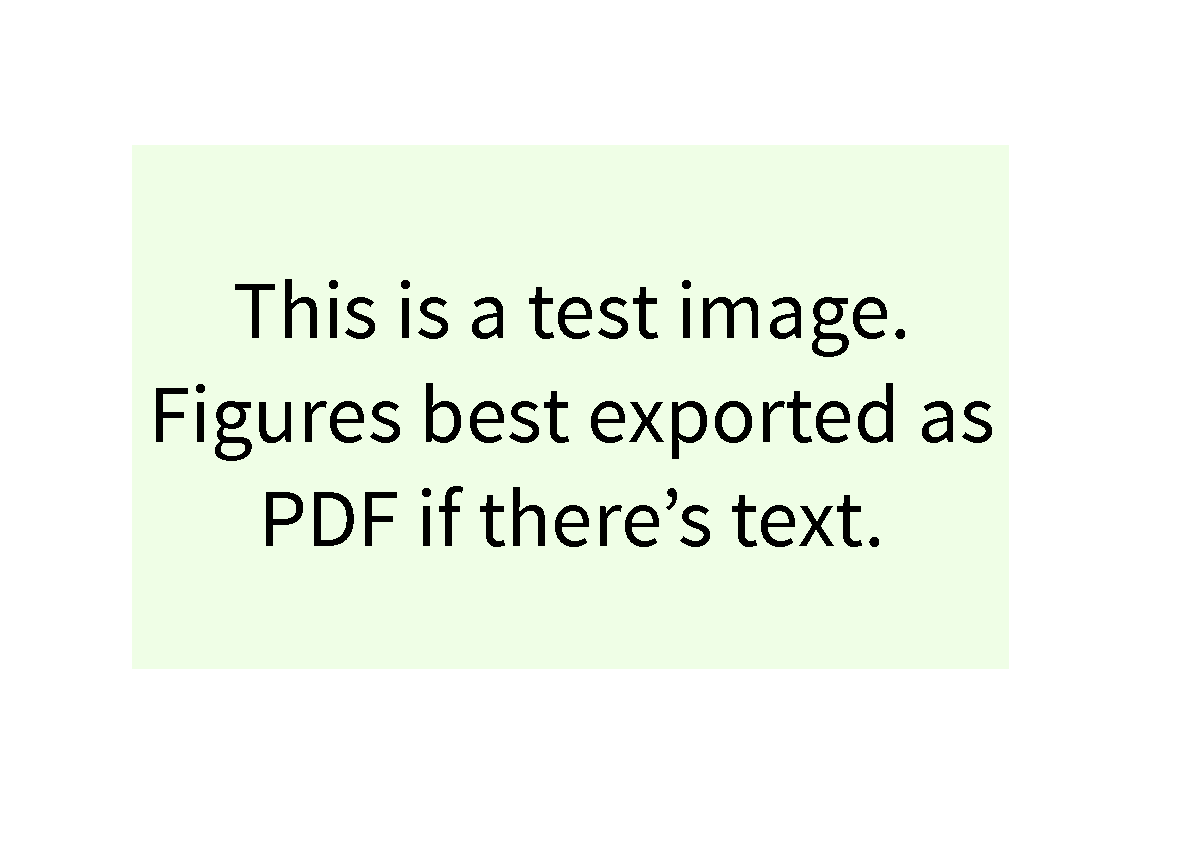
\includegraphics[width=6in]{images/template.pdf}
\caption{Sample figure}
\label{fig:sample-fig}
\end{figure}

\section{Numbered section once again}
At vero eos et accusamus et iusto odio dignissimos ducimus qui blanditiis praesentium voluptatum deleniti atque corrupti quos dolores et quas molestias excepturi sint occaecati cupiditate non provident, similique sunt in culpa qui officia deserunt mollitia animi, id est laborum et dolorum fuga. Et harum quidem rerum facilis est et expedita distinctio. Nam libero tempore, cum soluta nobis est eligendi optio cumque nihil impedit quo minus id quod maxime placeat facere possimus, omnis voluptas assumenda est, omnis dolor repellendus. Temporibus autem quibusdam et aut officiis debitis aut rerum necessitatibus saepe eveniet ut et voluptates repudiandae sint et molestiae non recusandae. Itaque earum rerum hic tenetur a sapiente delectus, ut aut reiciendis voluptatibus maiores alias consequatur aut perferendis doloribus asperiores repellat.

\begin{table}[]
\centering
\begin{tabularx}{\textwidth}{RRRRRR}
Col1 & Col2 & Col2 & Col3 \\
\hline
1 & 6 & 87837 & 787 \\ 
2 & 7 & 78 & 5415 \\
3 & 545 & 778 & 7507 \\
4 & 545 & 18744 & 7560 \\
5 & 88 & 788 & 6344 \\
\end{tabularx}
\caption{Sample table}
\label{tab:sample-table}
\end{table}

\end{document}